\documentclass{beamer}

\usetheme{Boadilla} % Escolha um tema
\usepackage{tikz}
\usetikzlibrary{positioning, arrows.meta}
\usepackage{pgfgantt}
\usepackage{graphicx}
\usepackage{adjustbox}
\usepackage{xcolor}
\usepackage{amsmath}
\usepackage{amssymb}
\usepackage{mathtools}
\usepackage{IEEEtrantools}
\usepackage{float}
\usepackage{booktabs}
\usepackage{multirow}
\usepackage[table]{xcolor}
\usepackage{adjustbox}

\title{O Problema da Compra Mínima: Heurísticas e Formulações}
\author{Antônio Erick Freitas Ferreira}
\institute{Unicamp}
\date{14 de Julho de 2026}

\newcommand{\conjuntoItens}{

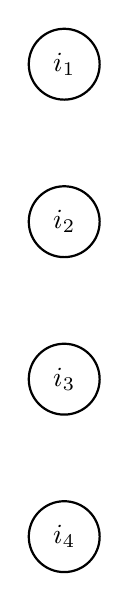
\begin{tikzpicture}[
    thick,
    item/.style={circle, draw, minimum size=9mm},
    buyer/.style={circle, draw,  minimum size=9mm}
]
    % Itens
    \node[item] (i1) at (0,2) {$i_1$};
    \node[item] (i2) at (0,0) {$i_2$};
    \node[item] (i3) at (0,-2) {$i_3$};
    \node[item] (i3) at (0,-4) {$i_4$};

\end{tikzpicture}
}


\newcommand{\conjuntoCompradores}{

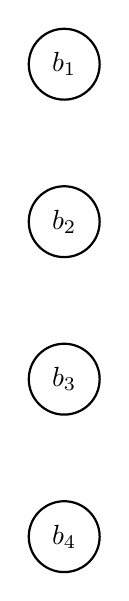
\begin{tikzpicture}[
    thick,
    item/.style={circle, draw, minimum size=9mm},
    buyer/.style={circle, draw,  minimum size=9mm}
]

    % Compradores
    \node[buyer] (b1) at (5,2) {$b_1$};
    \node[buyer] (b2) at (5,0) {$b_2$};
    \node[buyer] (b2) at (5,-2) {$b_3$};
    \node[buyer] (b2) at (5,-4) {$b_4$};

\end{tikzpicture}
}


\newcommand{\conjuntoItensValorados}{

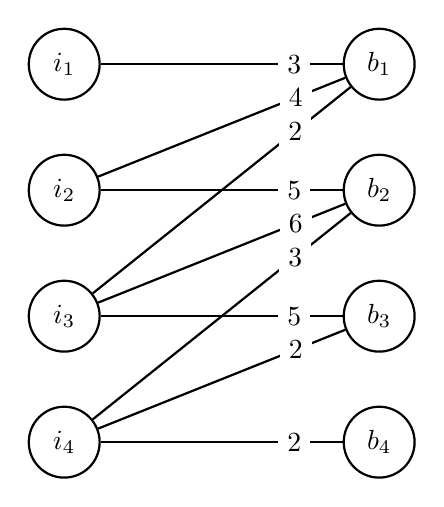
\begin{tikzpicture}[
    thick,
    item/.style={circle, draw, minimum size=9mm},
    buyer/.style={circle, draw,  minimum size=9mm},
    scale=0.8
]
    % Itens
    \node[item] (i1) at (0,2) {$i_1$};
    \node[item] (i2) at (0,0) {$i_2$};
    \node[item] (i3) at (0,-2) {$i_3$};
    \node[item] (i4) at (0,-4) {$i_4$};

    % Compradores
    \node[buyer] (b1) at (5,2) {$b_1$};
    \node[buyer] (b2) at (5,0) {$b_2$};
    \node[buyer] (b3) at (5,-2) {$b_3$};
    \node[buyer] (b4) at (5,-4) {$b_4$};

    % Arestas
    \draw (b1) --node[pos=0.2, fill=white]{3} (i1);
    \draw (b1) --node[pos=0.2, fill=white]{4} (i2);
    \draw (b1) --node[pos=0.215, fill=white]{2} (i3);

    \draw (b2) --node[pos=0.2, fill=white]{5} (i2);
    \draw (b2) --node[pos=0.2, fill=white]{6} (i3);
    \draw (b2) --node[pos=0.215, fill=white]{3} (i4);

    \draw (b3) --node[pos=0.2, fill=white]{5} (i3);
    \draw (b3) --node[pos=0.2, fill=white]{2} (i4);

    \draw (b4) --node[pos=0.2, fill=white]{2} (i4);
    % \draw (i2) -- (b2);
    % \draw (i3) -- (b2);
\end{tikzpicture}
}

\newcommand{\conjuntoItensPrecificados}{

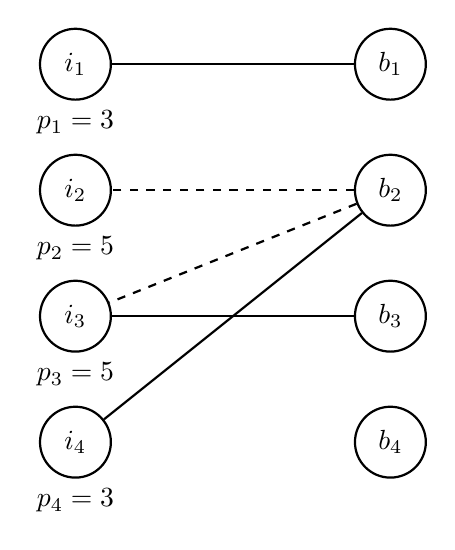
\begin{tikzpicture}[
    thick,
    item/.style={circle, draw, minimum size=9mm},
    buyer/.style={circle, draw,  minimum size=9mm},
    scale=0.8
]
    % Itens
    \node[item, label=below:{$p_1 = 3$}] (i1) at (0,2) {$i_1$};
    \node[item, label=below:{$p_2 = 5$}] (i2) at (0,0) {$i_2$};
    \node[item, label=below:{$p_3 = 5$}] (i3) at (0,-2) {$i_3$};
    \node[item, label=below:{$p_4 = 3$}] (i4) at (0,-4) {$i_4$};

    % Compradores
    \node[buyer] (b1) at (5,2) {$b_1$};
    \node[buyer] (b2) at (5,0) {$b_2$};
    \node[buyer] (b3) at (5,-2) {$b_3$};
    \node[buyer] (b4) at (5,-4) {$b_4$};

    % Arestas
    \draw (i1) -- (b1);
    \draw (i4) -- (b2);
    \draw (i3) -- (b3);


    % \draw[dashed, thick] (b1) -- (i2);
    % \draw[dashed, thick] (b1) -- (i3);

    \draw[dashed, thick] (b2) -- (i2);
    \draw[dashed, thick] (b2) --(i3);

    % \draw[dashed, thick] (b3) --(i4);

    % \draw[dashed, thick] (b4) -- (i4);
    
\end{tikzpicture}
}


\newcommand{\fluxograma}{
    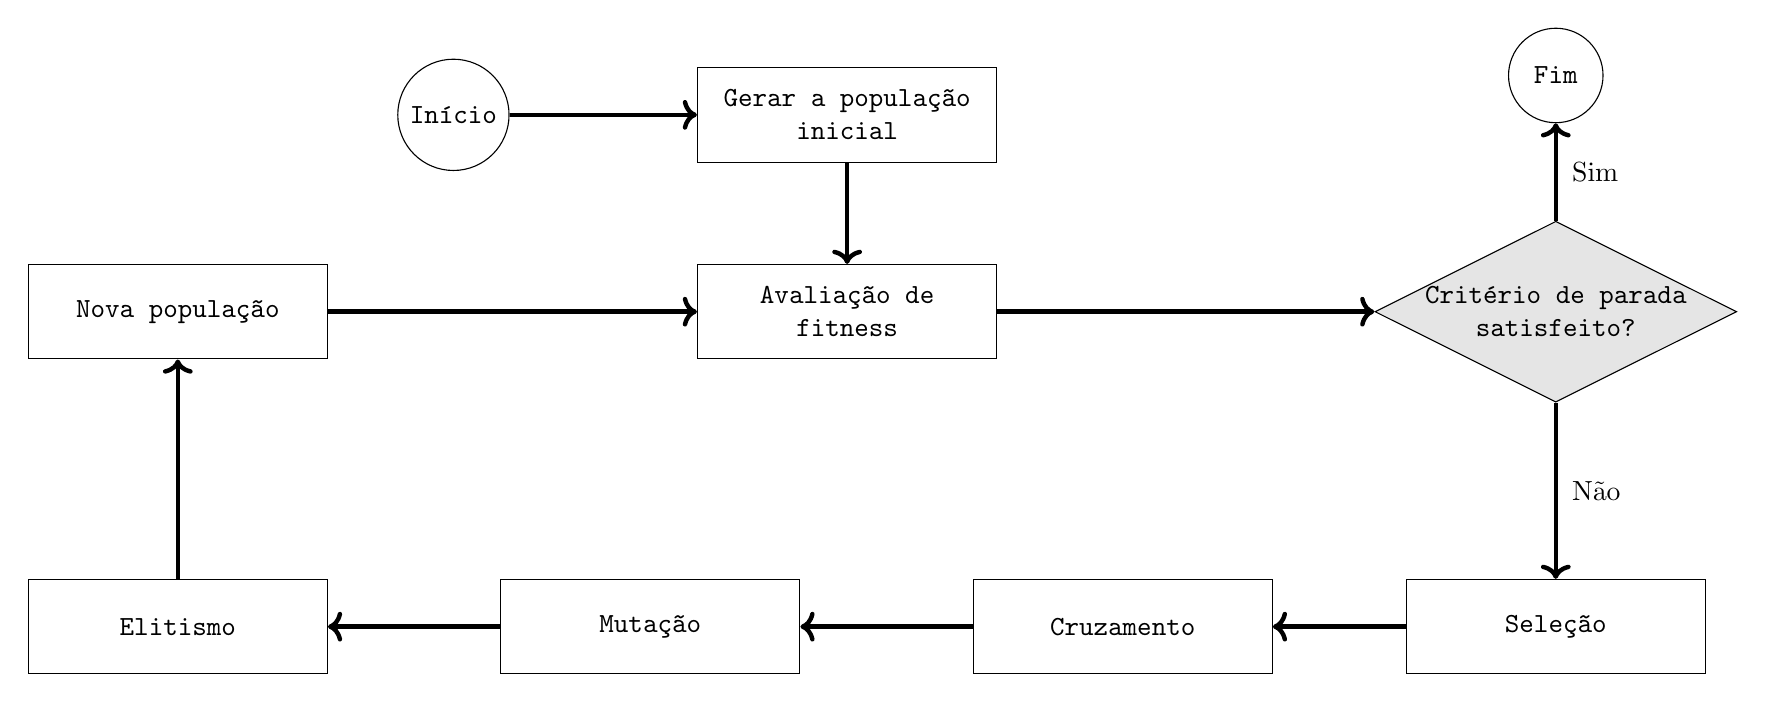
\begin{tikzpicture}[
        every node/.style={draw, minimum height=1.2cm, minimum width=3.8cm, font=\ttfamily, align=center},
        decision/.style={aspect=2, draw, minimum height=1.5cm, inner sep=0pt},
        arrow/.style={->, thick},
        node distance=1.2cm and 2cm
    ]
        % Nós
        \node (begin) at (-10,-1.5) [circle, draw, minimum size=1.2cm] {Início};
        \node (genKeys) at (-5,-1.5) {Gerar a população\\ inicial};
        \node (fitness) at (-5, -4) {Avaliação de \\ fitness};
        \node (checkStop) at (4, -4) [diamond, decision, fill=gray!20] {Critério de parada\\ satisfeito?};
        \node (selection) at (4, -8) {Seleção};
        \node (crossover) at (-1.5, -8) {Cruzamento};
        \node (mutation) at (-7.5, -8) {Mutação};
        \node (elitism) at (-13.5, -8) {Elitismo};
        \node (newPop) at (-13.5, -4) {Nova população};
        \node (final) at (4, -1) [circle, draw, minimum size=1.2cm] {Fim};
        
    \begin{scope}[
              every node/.style={fill=white,circle}, arrow/.style={->,ultra thick}]
        % Conexões
        \draw[arrow] (begin) -- (genKeys);
        \draw[arrow] (genKeys) -- (fitness);
        \draw[arrow] (fitness) -- (checkStop);
        \draw[arrow] (checkStop) --node[right]{Não} (selection);
        \draw[arrow] (selection) -- (crossover);
        \draw[arrow] (crossover) -- (mutation);
        \draw[arrow] (mutation) -- (elitism);
        \draw[arrow] (elitism) -- (newPop);
        \draw[arrow] (newPop) -- (fitness);
        \draw[arrow] (checkStop) -- node[right]{Sim} (final);
        
    \end{scope}
    \end{tikzpicture}
}

\newcommand{\fluxogramaBRKGA}{
    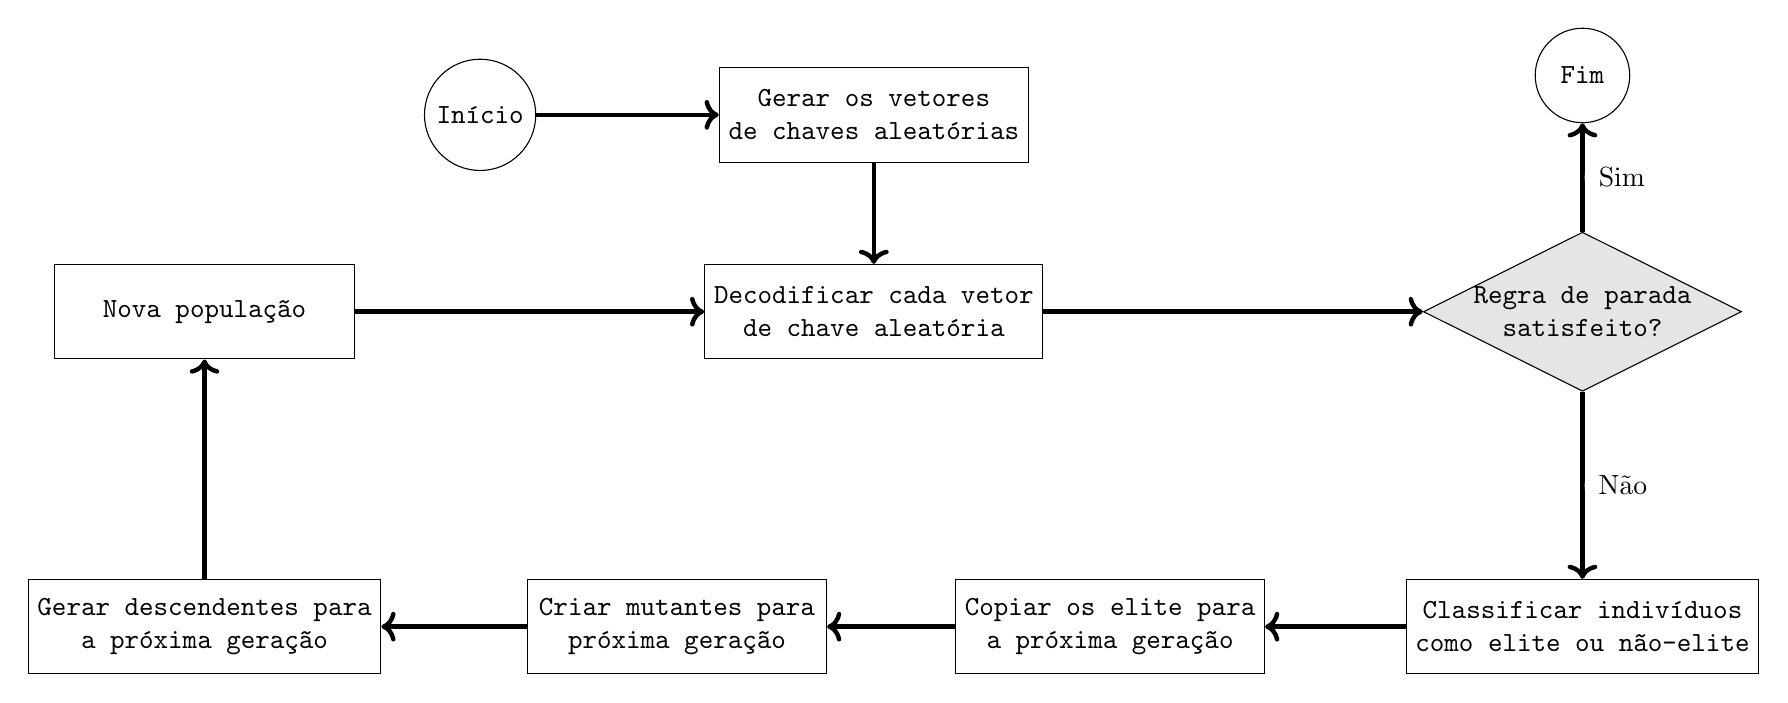
\begin{tikzpicture}[
        every node/.style={draw, minimum height=1.2cm, minimum width=3.8cm, font=\ttfamily, align=center},
        decision/.style={aspect=2, draw, minimum height=1.5cm, inner sep=0pt},
        arrow/.style={->, thick},
        node distance=1.2cm and 2cm
    ]
        % Nós
        \node (begin) at (-10,-1.5) [circle, draw, minimum size=1.2cm] {Início};
        \node (genKeys) at (-5,-1.5) {Gerar os vetores\\ de chaves aleatórias};
        \node (fitness) at (-5, -4) {Decodificar cada vetor \\ de chave aleatória};
        \node (checkStop) at (4, -4) [diamond, decision, fill=gray!20] {Regra de parada\\ satisfeito?};
        \node (selection) at (4, -8) {Classificar indivíduos\\como elite ou não-elite};
        \node (crossover) at (-2, -8) {Copiar os elite para\\a próxima geração};
        \node (mutation) at (-7.5, -8) {Criar mutantes para\\próxima geração};
        \node (elitism) at (-13.5, -8) {Gerar descendentes para\\a próxima geração};
        \node (newPop) at (-13.5, -4) {Nova população};
        \node (final) at (4, -1) [circle, draw, minimum size=1.2cm] {Fim};
        
    \begin{scope}[
              every node/.style={fill=white,circle}, arrow/.style={->,ultra thick}]
        % Conexões
        \draw[arrow] (begin) -- (genKeys);
        \draw[arrow] (genKeys) -- (fitness);
        \draw[arrow] (fitness) -- (checkStop);
        \draw[arrow] (checkStop) --node[right]{Não} (selection);
        \draw[arrow] (selection) -- (crossover);
        \draw[arrow] (crossover) -- (mutation);
        \draw[arrow] (mutation) -- (elitism);
        \draw[arrow] (elitism) -- (newPop);
        \draw[arrow] (newPop) -- (fitness);
        \draw[arrow] (checkStop) -- node[right]{Sim} (final);
        
    \end{scope}
    \end{tikzpicture}
}


\begin{document}

% Slide de título
\begin{frame}
    \titlepage
\end{frame}

% Slide comum
\begin{frame}{Introdução}

    \begin{center}
        
\includegraphics[width=0.7\textwidth]{../Texto/Secoes/Figuras/Photos/compra-venda.png}
    \end{center}
    \pause

    \begin{itemize}
        \item Rusmevichientong et al. (2006).
        % \item Guruswami et al. (2005)
    \end{itemize}
    

\end{frame}

\begin{frame}{Introdução}

    \begin{center}
        
\includegraphics[width=0.6\textwidth]{../Texto/Secoes/Figuras/Photos/compra-venda-imovel.jpg}
    \end{center}

    Possíveis comportamentos:
    \begin{itemize}
        \item Comportamento de compra máxima.
        \pause
        \item Comportamento de compra ranqueada.
        \pause
        \item \textcolor{green!50!black}{Comportamento de compra mínima}.
        \pause
        \item Comportamento de compra livre de inveja.
    \end{itemize}

\end{frame}

\begin{frame}{Introdução}

    \begin{columns}

        \column{0.48\textwidth}
        \centering
        \conjuntoItens

        \pause

        \column{0.48\textwidth}
        \centering
        \conjuntoCompradores

    \end{columns}

\end{frame}

\begin{frame}{Introdução}

    \begin{columns}

        \column{0.48\textwidth}
        \centering
        \conjuntoItensValorados
        \vspace*{6mm}
        \pause

        \column{0.48\textwidth}
        \centering
        \conjuntoItensPrecificados

    \end{columns}

\end{frame}

\begin{frame}{Introdução}

    Formalização do problema de compra mínima (PCmin):
    \begin{itemize}
        \item Conjunto de itens $I$.
        \pause
        \item Conjunto de compradores $B$.
        \pause
        \item Matriz de valorações $V = \{v_{ib} \mid v_{ib} \in \mathbb{R}_+\}$.
        \pause
        \item Cada comprador $b \in B$ escolhe o item de menor preço entre aqueles cujo preço é menor ou igual à sua valoração, ou não compra se nenhum item for viável.
        \pause
        \item O objetivo é determinar o conjunto $P = \{p_i \mid p_i \in \mathbb{R}_+, i \in I\} $ de preços.
    \end{itemize}

\end{frame}

\begin{frame}{Introdução}

    \begin{itemize}
        \item Do ponto de vista exato, Catabriga (2025) foi o primeiro a propor formulações de PLI e PLIM para o PCmin.
        \pause
        \item Do ponto de vista heurístico, não há trabalhos na literatura que abordem o PCmin.
    \end{itemize}

\end{frame}

\begin{frame}{Trabalhos Relacionados}
    
    \begin{itemize}
        \item Rusmevichientong et al. (2006).
        \pause
        \item Aggarwal et al. (2004).
        \pause
        \item Guruswami et al. (2005).
        \pause
        \item Heilporn et al. (2014) e Fernandes et al. (2015).
        \pause
        \item Briest e Krysta (2007).
        \pause
        \item Chalermsook et al. (2012).
        \pause
        \item Catabriga (2025).
    \end{itemize}

\end{frame}

\begin{frame}{Metodologia - Programação Linear}
    
    \begin{itemize}
        \item Técnica central da otimização combinatória
    \end{itemize}

    \[
        \begin{aligned}
        &\text{maximize} \quad  z  = &c^T x \\
        &\text{sujeito a} \quad & Ax & \leq  b \\
        & & x & \geq  0
        \end{aligned}
    \]

    em que:
    \begin{itemize}
        \item $x \in \mathbb{R}^n$ representa o vetor de variáveis de decisão;
        \item $c \in \mathbb{R}^n$ contém os coeficientes da função objetivo;
        \item $A \in \mathbb{R}^{m \times n}$ é a matriz de coeficientes das restrições;
        \item $b \in \mathbb{R}^m$ representa os termos independentes das restrições;
        \item $z \in \mathbb{R}$ é o valor da função objetivo.
    \end{itemize}
\end{frame}

\begin{frame}{Metodologia - Programação Linear}
    
    \begin{itemize}
        \item George Dantzig (1947) propôs o algoritmo simplex.
        \pause
        \item Leonid Khachiyan (1979) propôs o método dos elipsoides, provando que problemas de PL podem ser resolvidos em tempo polinomial.
        \pause
        \item Narendra Karmarkar (1984) propôs o método de pontos interiores.
    \end{itemize}

\end{frame}

\begin{frame}{Metodologia - Programação Linear Inteira e Inteira Mista}
    
    \begin{itemize}
        \item Impõe restrições de integralidade sobre algumas ou todas as variáveis de decisão.
        \pause
        \item Problemas de PLI e PLIM são NP-difíceis.
        \pause
        \item Algoritmos sofisticados: Branch-and-Bound e Branch-and-Cut.
        \pause
        \item Relaxação linear.
    \end{itemize}

\end{frame}

\begin{frame}{Metodologia - Algoritmo Genético}
    
    \begin{center}
        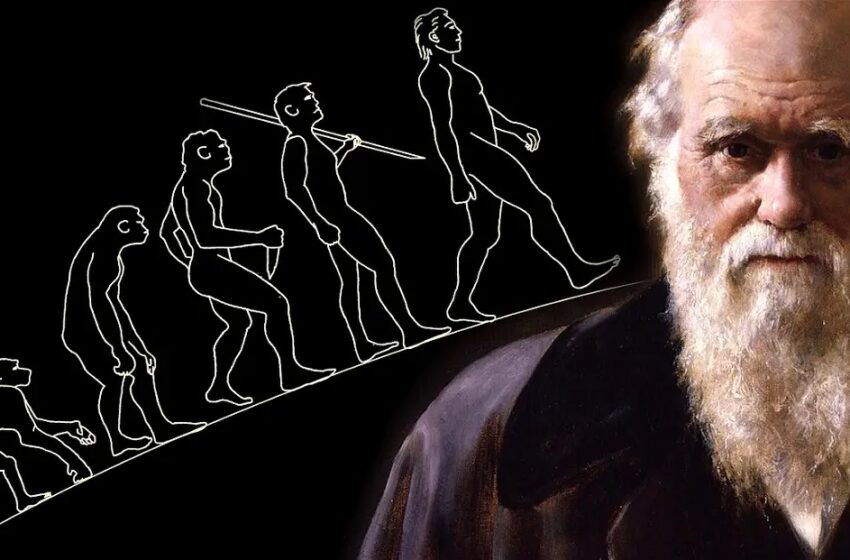
\includegraphics[width=0.5\textwidth]{../Texto/Secoes/Figuras/Photos/darwin.jpg}
    \end{center}
    \pause
    \begin{itemize}
        \item Algoritmos genéticos (GA).
    \end{itemize}

\end{frame}

\begin{frame}{Metodologia - Algoritmo Genético}

\centering

\resizebox{\textwidth}{!}{
    \fluxograma
}

\end{frame}

\begin{frame}{Metodologia - BRKGA}

    \begin{itemize}
        \item Extensão do RKGA, proposto por Bean (1994).
        \pause
        \item Uma solução é representada por um vetor de chaves aleatórias no intervalo $[0,1)$ e depois é interpretado por um decodificador específico.
        \pause
        \item No BRKGA, a população é dividida em três grupos: elite, mutantes e filhos. 
        \pause
        \item O crossover é feito entre indivíduos elite e não-elite, com maior probabilidade de herdar o gene do indivíduo elite.
        \pause
        \item O BRKGA é capaz de evitar estagnação prematura adotando estratégias de reinicialização da população.
    \end{itemize}

\end{frame}

\begin{frame}{Metodologia - BRKGA}

\centering

\resizebox{\textwidth}{!}{
    \fluxogramaBRKGA
}

\end{frame}

\begin{frame}{Metodologia - RKO}

    \begin{itemize}
        \item É um framework que generaliza o paradigma das chaves aleatórias desacoplando-a da estrututra do GA.
        \pause
        \item O RKO permite que diferentes meta-heurísticas operem diretamente no espaço contínuo das chaves aleatórias, permitindo que um decodificador seja usado por diferentes estratégias de busca.
        \pause
        \item O elemento central do RKO é o elite pool.
    \end{itemize}

\end{frame}

\begin{frame}{Metodologia - RKO}

    \begin{center}
        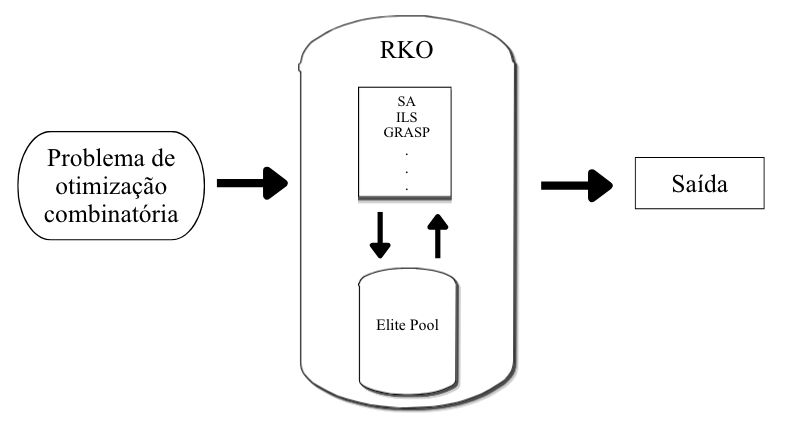
\includegraphics[width=0.8\textwidth]{../Texto/Secoes/Figuras/Photos/RKO_FLOW_V3.jpeg}
    \end{center}

\end{frame}

\begin{frame}{Formulações matemáticas da literatura}

    \begin{itemize}
        \item Formulação de Decisão Indireta Binária (DIB).
        \item Formulação de Decisão Direta (DD).
        \pause
        \item \textbf{Teorema 2:} Prova que o conjunto de preços $P$ é um subconjunto do conjunto de valorações $V$.
    \end{itemize}

\end{frame}

\begin{frame}[shrink]{Formulações matemáticas da literatura - DIB}

    \begin{itemize}
        \item $x_{ip}$ indica se o item $i$ recebe o preço $p$.
        \item $y_{bp}$ indica se o comprador $b$ realiza uma compra pagando o valor $p$.
    \end{itemize}
    \pause
    \footnotesize

    \begin{align}
    \textbf{(DIB)}\qquad
    \max\quad & \sum_{b\in B}\sum_{p\in P} p\,y_{bp} \notag\\[0.4em]
    \text{s.a.}\quad
    &\sum_{p\in P}x_{ip}\le1, && \forall i\in I, \label{eq:dib1}\\
    &y_{bp}\le \sum_{\substack{i\in I\\ p\le v_{ib}}}x_{ip}, && \forall b\in B,\; \forall p\in P, \label{eq:dib2}\\
    &\sum_{p\in P}y_{bp}\le1, && \forall b \in B, \label{eq:dib3}\\
    &\sum_{\substack{p'<p\\ p'\le v_{ib}}} x_{ip'} \le 1-y_{bp}, && \forall b\in B,\; \forall i\in I,\; \forall p\in P, \label{eq:dib4}\\
    &x_{ip},\,y_{bp}\in\{0,1\}, && \forall i\in I,\; \forall b\in B,\; \forall p\in P. \label{eq:dib5}
    \end{align}


\end{frame}

\begin{frame}[shrink]{Formulações matemáticas da literatura - DD}
    \begin{center}
        
        \begin{itemize}
            \item $x_{ip}$ indica se o item $i$ recebe o preço $p$.
            \item $y_{ib}$ indica se o item $i$ é viável para o comprador $b$ cosiderando o preço $\pi_i$.
            \item $\pi_i$ indica o preço do item $i$.
            \item $\hat{p}_{ib}$ indica o valor pago pelo comprador $b$ ao adquirir o item $i$.
            \item $S_b$ indica os itens de interesse do comprador $b$.
            \item $R_i$ indica a maior valoração do item $i$.
            \item $R_b$ indica o maior valor associado pelo comprador $b$ a um item de seu interesse.
            \item $\epsilon$ indica a menor diferença positiva dentre todas as valorações.
        \end{itemize}
    \end{center}

\end{frame}


\begin{frame}[shrink]{Formulações matemáticas da literatura - DD}
    \footnotesize
    \begin{alignat}{3}
    \textbf{(DD)} \quad
    &\max \quad && \sum_{b \in B} \sum_{i \in S_b} \hat{p}_{ib}\\
    &\text{sujeito a} \quad
    && \sum_{i \in S_b} x_{ib} \leq 1, \quad && \forall b \in B \label{dd_1}\\
    & && v_{ib}\,x_{ib} - \hat{p}_{ib} \geq 0, \quad && \forall b \in B,\;\forall i \in S_b \label{dd_2}\\
    & && \hat{p}_{ib} \leq \pi_i, \quad && \forall b \in B,\;\forall i \in S_b \label{dd_3}\\
    & && \hat{p}_{ib} \geq \pi_i - R_i(1 - x_{ib}), \quad && \forall b \in B,\;\forall i \in S_b \label{dd_4}\\
    & && y_{ib} \geq \frac{v_{ib} - \pi_i + \epsilon}{v_{ib} + \epsilon}, \quad && \forall b \in B,\;\forall i \in S_b \label{dd_viab}\\
    & && \pi_i \geq \sum_{j \in S_b} \hat{p}_{jb} - R_b(1 - y_{ib}), \quad && \forall b \in B,\;\forall i \in S_b \label{dd_pcm}\\
    & && \hat{p}_{ib} \geq 0, \quad && \forall b \in B,\;\forall i \in S_b \label{dd_5}\\
    & && \pi_i \geq 0, \quad && \forall i \in I \label{dd_6}\\
    & && x_{ib},\,y_{ib} \in \{0,1\}, \quad && \forall b \in B,\;\forall i \in S_b \label{dd_7}
    \end{alignat}

\end{frame}

\begin{frame}{Objetivos}
    
    \begin{enumerate}
        \item Investigar e aperfeiçoar as formulações matemáticas existentes para o PCmin.
        \pause
        \item Desenvolver heurísticas baseadas nas abordagens BRKGA e RKO.
    \end{enumerate}

\end{frame}

% Slide com equação
\begin{frame}{Plano de trabalho}
    \begin{table}
    \label{cronograma}
    \centering
    \begin{adjustbox}{width=\textwidth}
    \begin{tabular}{l ccc cccc c}
    \toprule
    & \multicolumn{8}{c}{\textbf{Meses}} \\
    \cmidrule{2-9}
    & \textbf{1º - 3º} & \textbf{4º - 6º} & \textbf{7º - 9º} & \textbf{10º - 12º} & \textbf{13º - 15º} & \textbf{16º - 18º} & \textbf{19º - 21º} & \textbf{22º - 24º} \\
    \midrule
    Disciplinas                   & • & • & • & • &   &   &   &   \\
    EQM                           &   &   & • &   &   &   &   &   \\
    Revisão bibliográfica        & • & • &   &   &   &   &   &   \\
    % BEPE                          &   &   &   &   & • & • &   &   \\
    PED                           &   &   &  &  & • & • &   &   \\
    Desenvolvimento de formulações     &   &   & • & • & • &   &   &   \\
    Desenvolvimento de heurísticas&   &   &   &   &  & • & •  &  • \\
    Experimentação computacional  &   &   & • & • & • & • & • &  • \\
    % Escrita de artigos científicos&   &   &   &   &   &   & • &   \\
    Escrita de artigos científicos e dissertação        &   &   &   &   &   &   &   & • \\
    % Entrega da dissertação e defesa&  &   &   &   &   &   &   & • \\
    \bottomrule
    \end{tabular}
    \end{adjustbox}
    \end{table}
\end{frame}

\begin{frame}{Materiais e métodos}
    
    \begin{enumerate}
        \item Desenvolvimento no Laboratório de Otimização e Combinatória (LOCo) do Instituto de Computação.
        \pause
        \item Experimentos computacionais serão executados nos servidores de alto desempenho do LOCo.
        \pause
        \item Suporte teórico e levantamento do estado da arte, será usado a biblioteca do IMECC e o Portal de Periódicos da CAPES.
        \pause
        \item Será realizado reuniões com o orientador além de reuniões periódicas com os demais membros do grupo de pesquisa do orientador.
    \end{enumerate}

\end{frame}

\begin{frame}{Forma de análise dos resultados}
    
    \begin{enumerate}
        \item As formulações matemáticas serão avaliadas por sua capacidade de produzir soluções ótimas ou limites de alta qualidade dentro de tempos preestabelecidos.
        \pause
        \item Também será avaliado a consistência dos modelos em cenários de diferentes dimensões.
        \pause
        \item Para comparar as diferentes formulações, será utilizado a metodologia de \emph{performance profile}.
        \pause
        \item Os resultados das heurísticas serão comparados com os resultados obtidos pelos métodos exatos quando possível, quando não, a avaliação será complementada por meio de \emph{performance profile}.
        \pause
        \item Para avaliar o comportamento estocástico das heurísticas, será usado a metodologia de \emph{Time-to-Target}.
        \pause
        \item Por fim, as análises serão consolidadas em artigos científicos e na dissertação de mestrado.
    \end{enumerate}

\end{frame}

% Slide com figura
\begin{frame}
\begin{center}
    Obrigado!
\end{center}
\end{frame}

\end{document}